%Correct the file name.
%X: book number
%Y: part number
%ZZZ: page number in three digits. So page 3 would be 003.

\documentclass[11pt]{amsbook}

\usepackage{../HBSuerDemir}	% ------------------------


\begin{document}

% ++++++++++++++++++++++++++++++++++++++
\hPage{b2p2/481}
% ++++++++++++++++++++++++++++++++++++++

\noindent and the tangent line is equal to the square of the radius 
vector. \\
\noindent 39. Find the equation of the curves such that its slope at any 
point $P\hPairingParan{x,y}$ is equal to the difference of the squares of the distances of $P\hPairingParan{x,y}$ from the points $\hPairingParan{1,0}$ and $\hPairingParan{4,0}$.

\noindent 40. Find the orthogonal trajectories of the following family:\\
\begin{tabular}{cc}
a) $y^2=4ax$, \quad \quad \quad \quad 
b) $xy=c$
\end{tabular}


\noindent 41. Same question for:\\
\begin{tabular}{cc}
a) $r= c \cos\theta$, \quad \quad \quad \quad 
b) $\hPairingParan{1+2\cos\theta}r=2$
\end{tabular}\\
\noindent 42. Same question for:\\
\begin{tabular}{cc}
a) $2x^2+3y^2=c$,  \quad \quad 
b) $x^2+y^2=cx$
\end{tabular}\\
\noindent 43. Find the stream line through $A\hPairingParan{3,1}$ of the vector field:
$$
F=\hPairingParan{2xy,x^2-y^2}
$$

\noindent 44. The surface area A of a snowball increases proportional to the area at that moment. If $A=4\pi$ $dm^2$ at $t= 0$ and $64\pi$  $dm^2$ at $t = 2$ min, find the area at $t = 3$ min.\\
\noindent 45.  A body falls from rest through air. If air resistance is proportional to the square of the velocity, determine its equation of motion $s=s(t)$. 
\section*{ANSWERS}
\noindent 36. $yy\prime^2+2xy\prime-y=0$
\\ \noindent 37. $y^2=6x+10$
\\ \noindent 38. $r^2=\pm20+c$
\end{document}  

%==== templates ====

%==== environments ====

%\begin{figure}[htb]
%	\centering
%	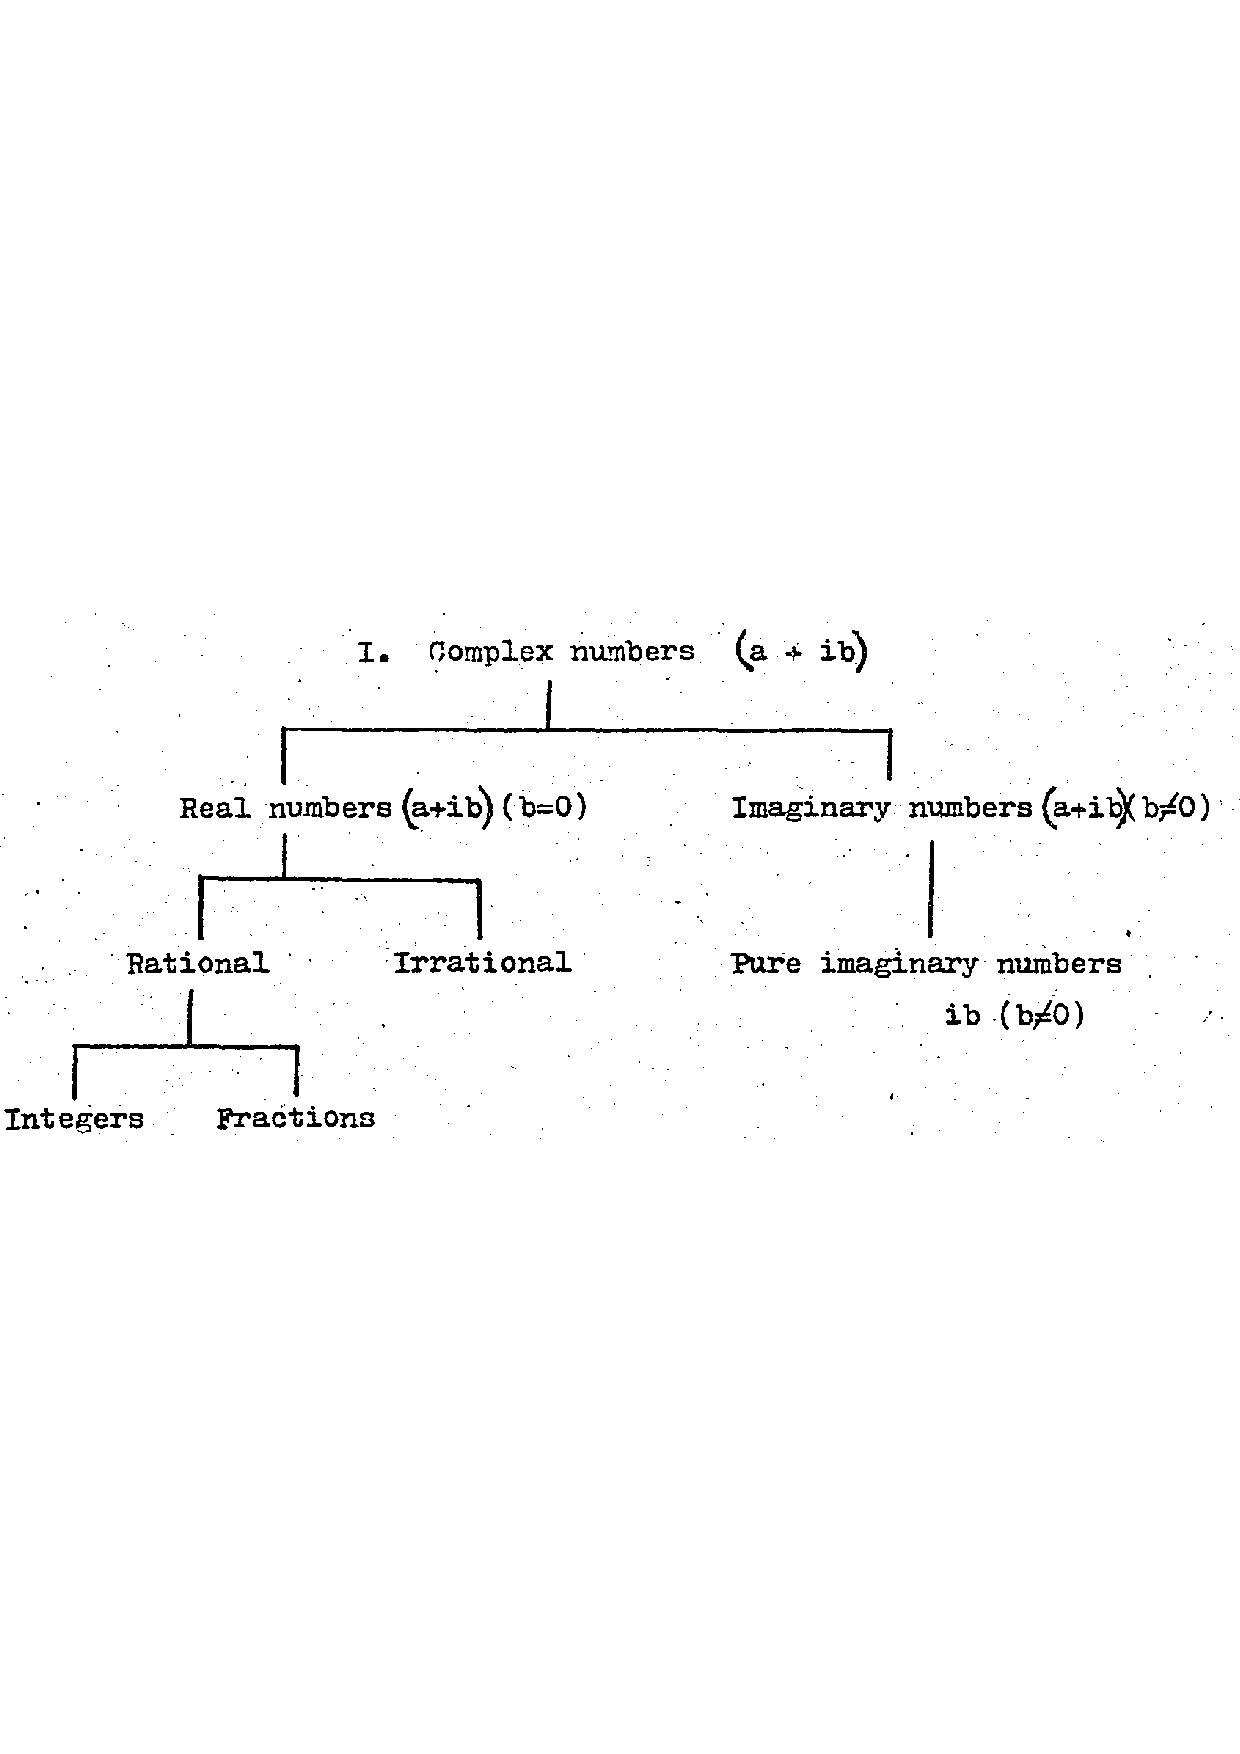
\includegraphics[width=0.9\textwidth]{images/SD-1-1p15A}
%	\caption{Classification of complex numbers}
%	\label{fig:classificationOfComplexNumbersA}
%\end{figure}

%\begin{center}
%\begin{tabular}{cc}
%\end{tabular}
%\end{center}

%\begin{exmp}
%\begin{hSolution}
%\end{hSolution}
%\end{exmp}

%\begin{hEnumerateAlpha}
%\end{hEnumerateAlpha}

%\begin{hEnumerateRoman}
%\end{hEnumerateRoman}

%$
%\begin{bmatrix}
%\end{bmatrix}
%$

%\frac{aaaa}{bbb}
%\frac{a_{n}}{b_{n}}
%\left( aaaa \right)
%\Longrightarrow

%\begin{multicols}{2}
%	bb
%\columnbreak
%	aa
%\end{multicols}
